%!TEX program = xelatex


\documentclass[9pt,twocolumn,twoside]{pnas-new}
% Use the lineno option to display guide line numbers if required.
% Note that the use of elements such as single-column equations
% may affect the guide line number alignment. 

\templatetype{pnasresearcharticle} % Choose template 
% {pnasresearcharticle} = Template for a two-column research article
% {pnasmathematics} = Template for a one-column mathematics article
% {pnasinvited} = Template for a PNAS invited submission

\usepackage{csvsimple}
% \usepackage{subcaption}
% \usepackage{csquotes}

\title{Diversity, Segregation, and Information in Cities}

% Use letters for affiliations, numbers to show equal authorship (if applicable) and to indicate the corresponding author
\author[a,b,1]{Philip Chodrow}

\affil[a]{Human Mobility and Networks Laboratory, Massachusetts Institute of Technology, Cambridge, MA 02139}
\affil[b]{Operations Research Center, Massachusetts Institute of Technology, Cambridge, MA 02139}

% Please give the surname of the lead author for the running footer
\leadauthor{Chodrow} 

% Please add here a significance statement to explain the relevance of your work
\significancestatement{Authors must submit a 120-word maximum statement about the significance of their research paper written at a level understandable to an undergraduate educated scientist outside their field of speciality. The primary goal of the Significance Statement is to explain the relevance of the work in broad context to a broad readership. The Significance Statement appears in the paper itself and is required for all research papers.}

% Please include corresponding author, author contribution and author declaration information
% \authorcontributions{Please provide details of author contributions here.}
\authordeclaration{The author declares no competing interest.}
% \equalauthors{\textsuperscript{1}A.O.(Author One) and A.T. (Author Two) contributed equally to this work (remove if not applicable).}
\correspondingauthor{\textsuperscript{1}To whom correspondence should be addressed. E-mail: pchodrow@gmail.com}

% Keywords are not mandatory, but authors are strongly encouraged to provide them. If provided, please include two to five keywords, separated by the pipe symbol, e.g:
\keywords{Information Theory $|$ Diversity and Segregation $|$ Urban Theory } 

\begin{abstract}
Please provide an abstract of no more than 250 words in a single paragraph. Abstracts should explain to the general reader the major contributions of the article. References in the abstract must be cited in full within the abstract itself and cited in the text.
\end{abstract}

\dates{This manuscript was compiled on \today}
\doi{\url{www.pnas.org/cgi/doi/10.1073/pnas.XXXXXXXXXX}}

\begin{document}

% Optional adjustment to line up main text (after abstract) of first page with line numbers, when using both lineno and twocolumn options.
% You should only change this length when you've finalised the article contents.
\verticaladjustment{-2pt}

\maketitle
\thispagestyle{firststyle}
\ifthenelse{\boolean{shortarticle}}{\ifthenelse{\boolean{singlecolumn}}{\abscontentformatted}{\abscontent}}{}

% If your first paragraph (i.e. with the \dropcap) contains a list environment (quote, quotation, theorem, definition, enumerate, itemize...), the line after the list may have some extra indentation. If this is the case, add \parshape=0 to the end of the list environment.
\dropcap{I}nformation theory...blah blah blah. 

	\begin{figure}%[tbhp]
		\centering % need to center this
		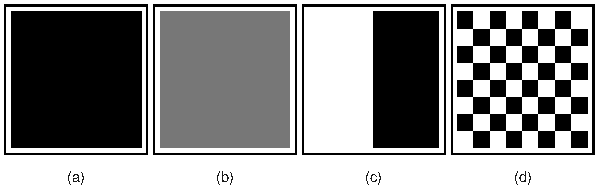
\includegraphics[width=\linewidth]{figs/checkerboard.pdf}
		\caption{
			Schematic cities illustrating three dimensions of segregation. 
			City (a) lacks global diversity, while Cities (b)-(d) are maximally globally diverse. 
			City (b) is perfectly spatially even, whereas Cities (c) and (d) are maximally uneven. 
			City (d) has higher spatial exposure than City (c) due to more contact points between racially distinct neighborhoods.
		} \label{fig:checkerboard}
	\end{figure}


\section*{Results}


	\begin{figure}
			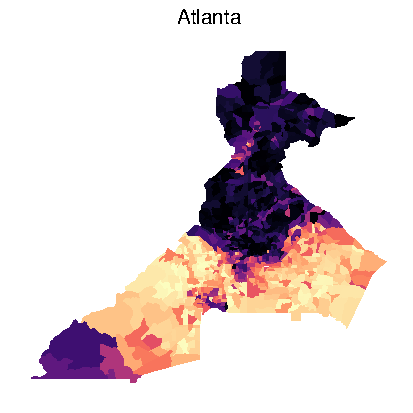
\includegraphics[width = .5\linewidth]{figs/Atlanta_percent_black.pdf}
			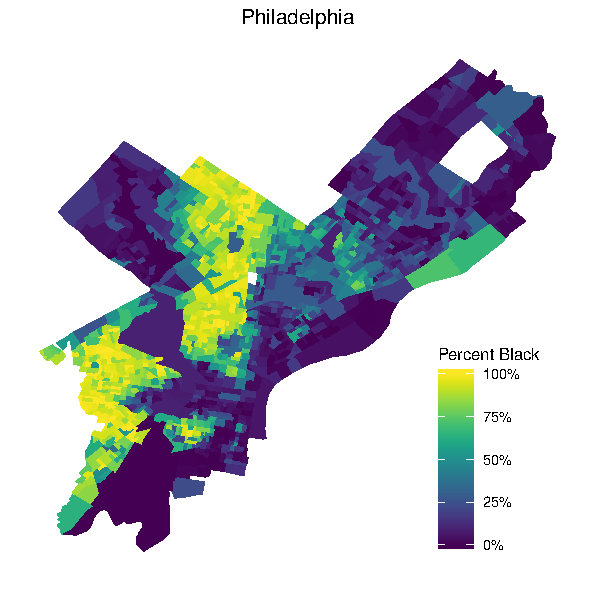
\includegraphics[width = .5\linewidth]{figs/Philadelphia_percent_black.pdf} \\
			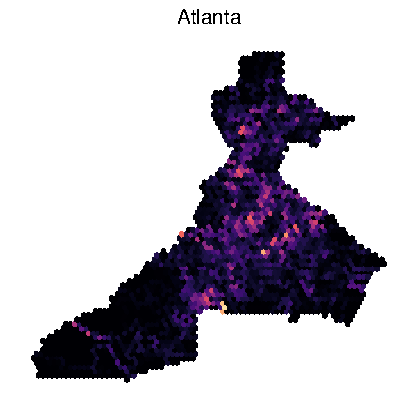
\includegraphics[width = .5\linewidth]{figs/Atlanta_grid.pdf} 
			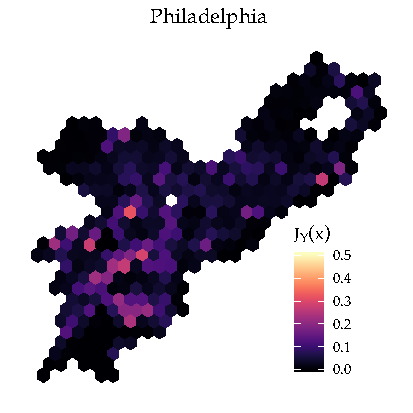
\includegraphics[width = .5\linewidth]{figs/Philadelphia_grid.pdf} \\

			\centering
			\begin{tabular}{l | c c c c}
				\bfseries City & Percent Black & $H(Y)$ & $I(X,Y)$ & $J(X,Y)$  \\\hline
				\csvreader[late after line=\\]{figs/comparative_summary.csv}{}
				{\csvcoli & \csvcolii & \csvcoliii & \csvcoliv & \csvcolv}
			\end{tabular}

			\caption{
				Spatial analysis of residential segregation in Atlanta (left) and Philadelphia (right). 
				(\emph{Top}): Percentage of black residents. 
				(\emph{Middle}): Hexgrid of spatial resolution 1km imposed over each city, shaded by the value of the local information $I(X,Y | X \in B_i)$. 
				(\emph{Bottom}): Numerical summary, including the three information measures.
			} \label{fig:Atlanta_philly}
	\end{figure}


	\begin{figure}
		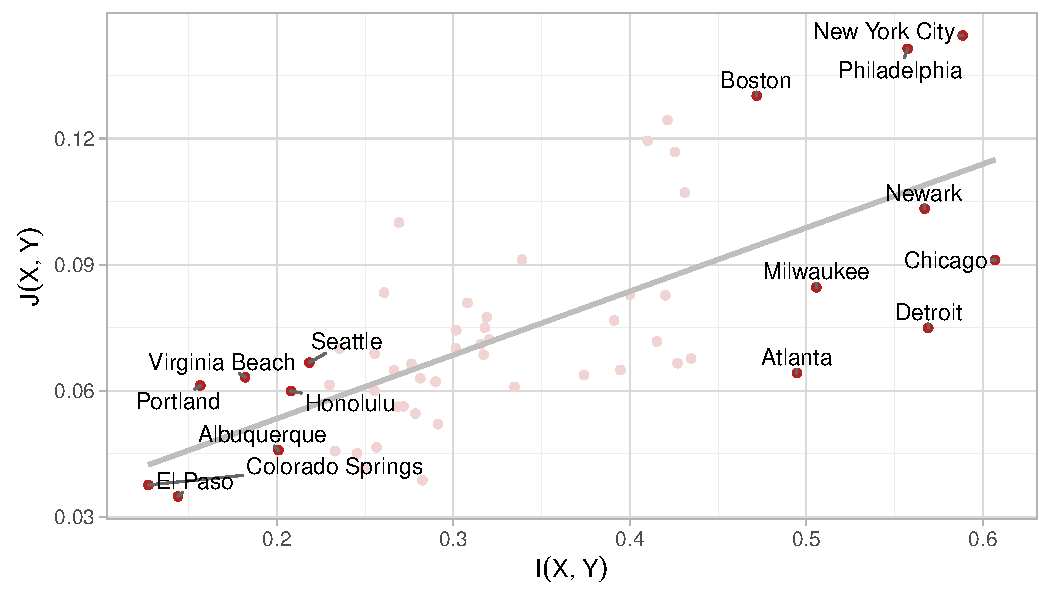
\includegraphics[width=\linewidth]{figs/mutual_fisher.pdf}
		\caption{
			Comparative global segregation measures in major U.S. cities, measured using racial categories $\mathcal{Y} = \{\text{Asian }, \text{Black }, \text{Hispanic }, \text{Other }, \text{White}\}$. 
			We used a hexgrid of spatial resolution $r = 1$km for the computation of $J(X,Y)$.
		} \label{fig:mutual_fisher}
	\end{figure}



\subsection*{Using some damn math} 
There's lots of damn math we could use. 

	\begin{figure}

		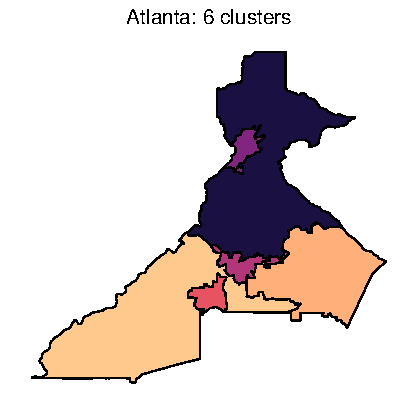
\includegraphics[width = .5\linewidth]{figs/Atlanta_clusters_binary_6.pdf} 
		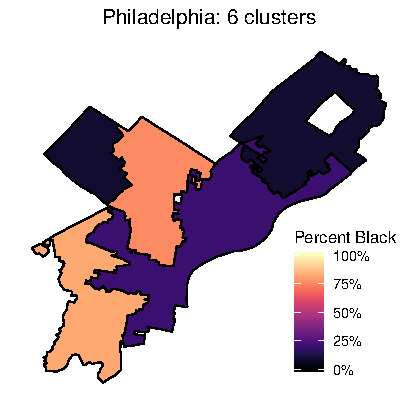
\includegraphics[width = .5\linewidth]{figs/Philadelphia_clusters_binary_6.pdf} \\
		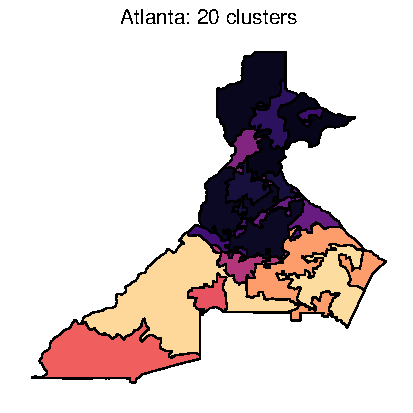
\includegraphics[width = .5\linewidth]{figs/Atlanta_clusters_binary_20.pdf}
		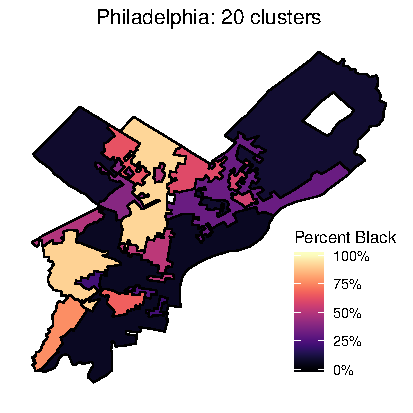
\includegraphics[width = .5\linewidth]{figs/Philadelphia_clusters_binary_20.pdf} \\
		
		\centering
		\begin{tabular}{l | c c c}
			\bfseries City  & $I(C_6, Y)$ & $I(C_{20},Y)$ & $I(X,Y)$ \\\hline
			\csvreader[late after line=\\]{figs/clustering_summary.csv}{}
			{\csvcoli & \csvcoliii & \csvcoliv & \csvcolii}
		\end{tabular}
		\caption{
			Example clusterings in Atlanta and Philadelphia using \eqref{eq:cluster_opt}, using $6$ and $20$ clusters. 
			The table below summarizes the between-groups mutual information captured by each cluster and compares it to the mutual information in the unaggregated blockgroup level data.
		} \label{fig:clusterings}

	\end{figure}

	\begin{figure}
		\centering
			% \begin{subfigure}[b]{0.45\linewidth}
			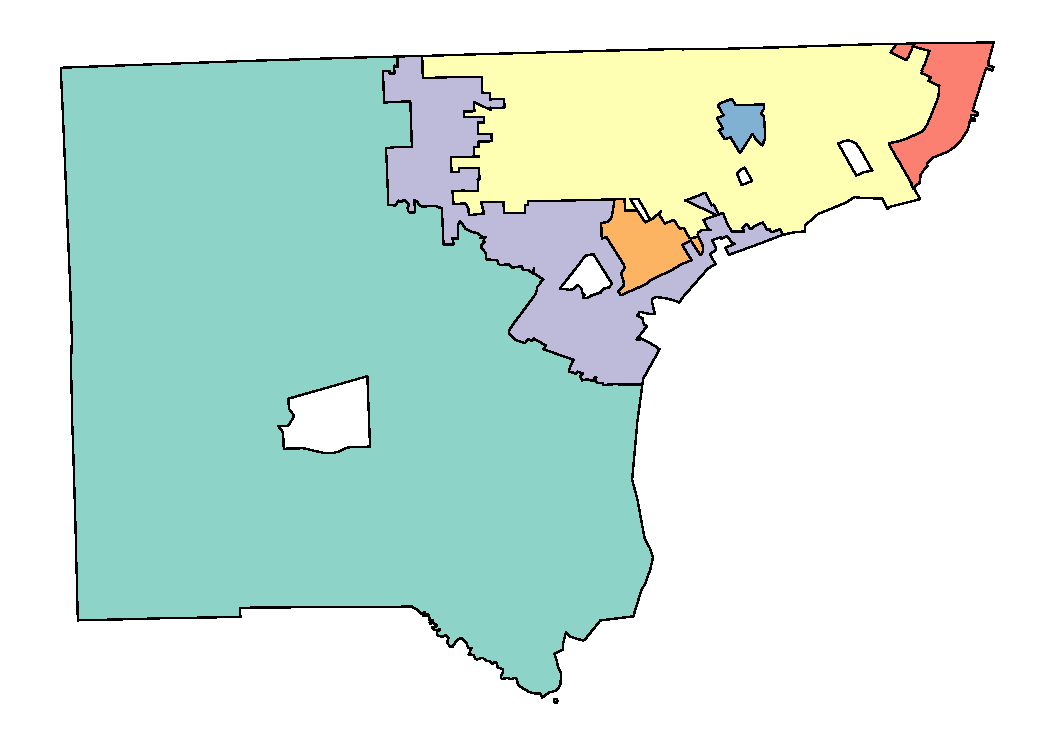
\includegraphics[width = .4\linewidth]{figs/example_cluster_map.pdf}
			% \caption{} \label{subfig:detroit_map}
			% \end{subfigure}
			% \begin{subfigure}[b]{0.45\linewidth}
			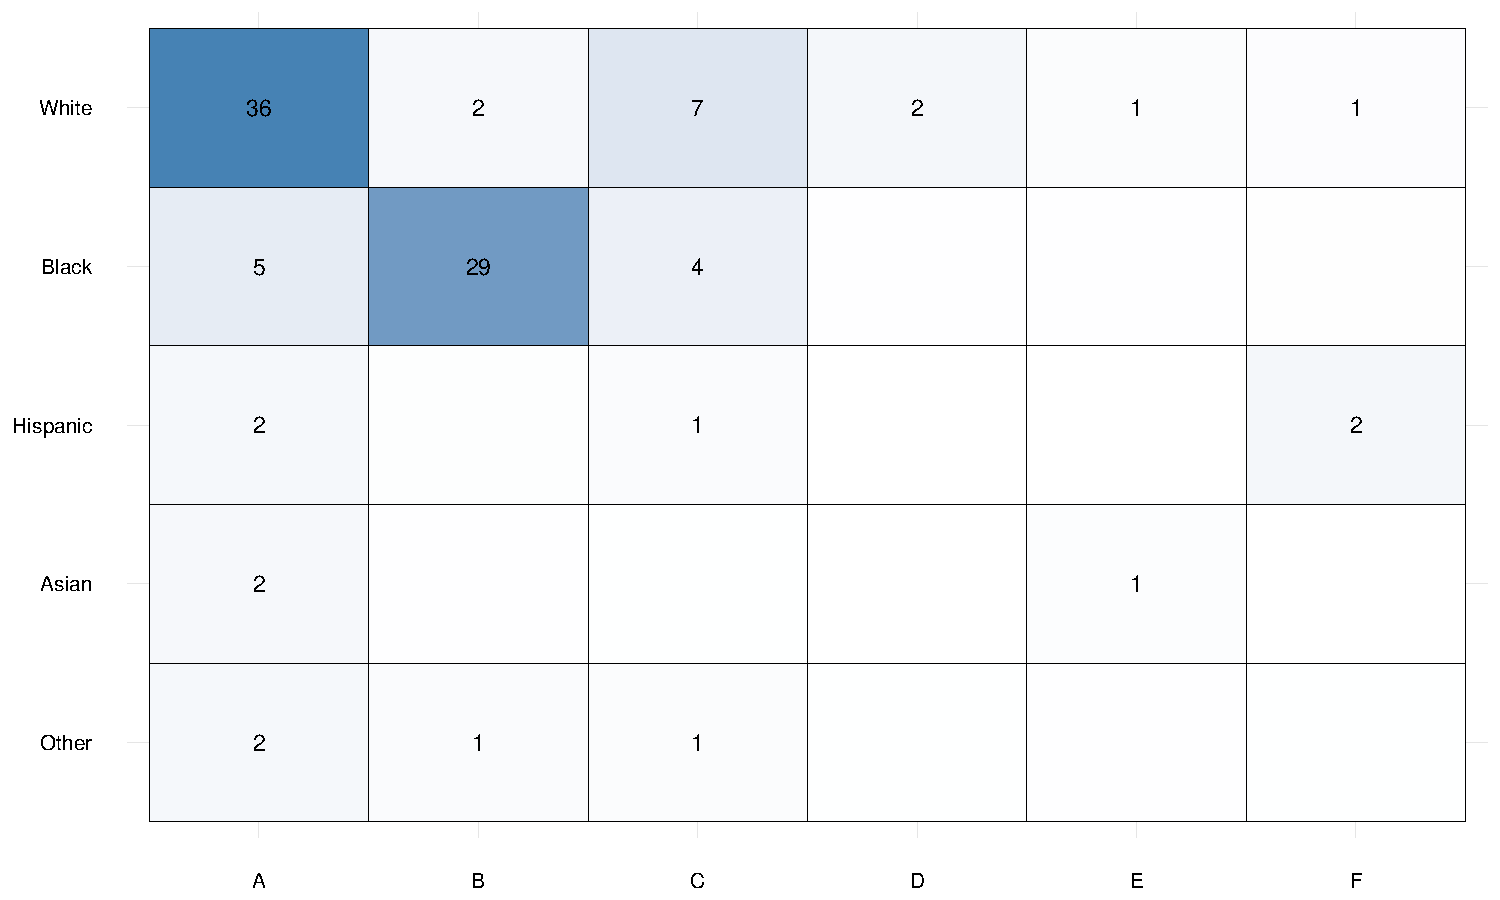
\includegraphics[width = .4\linewidth]{figs/example_clusters_detailed.pdf}
			% \caption{} \label{subfig:detroit_groups}
			% \end{subfigure}
			\caption{
				Multigroup sociospatial structure in Detroit. 
				\ref{subfig:detroit_map}: Map of six clusters. 
				\ref{subfig:detroit_groups}: Joint distribution of demographics and clusters. 
				Shadings reflect population proportions within clusters. 
				Numerical labels give raw population proportions; for example, 29\% of the population is Black and resides in cluster B. 
				Detroit has $H(Y) = 1.12$, $I(X,Y) = 0.57$, and $J(X,Y) = 0.08$. 
				This clustering captures $I(C_6,Y) = 0.36$ nats of information.
			} \label{fig:detroit}
	\end{figure}


	\begin{figure}
			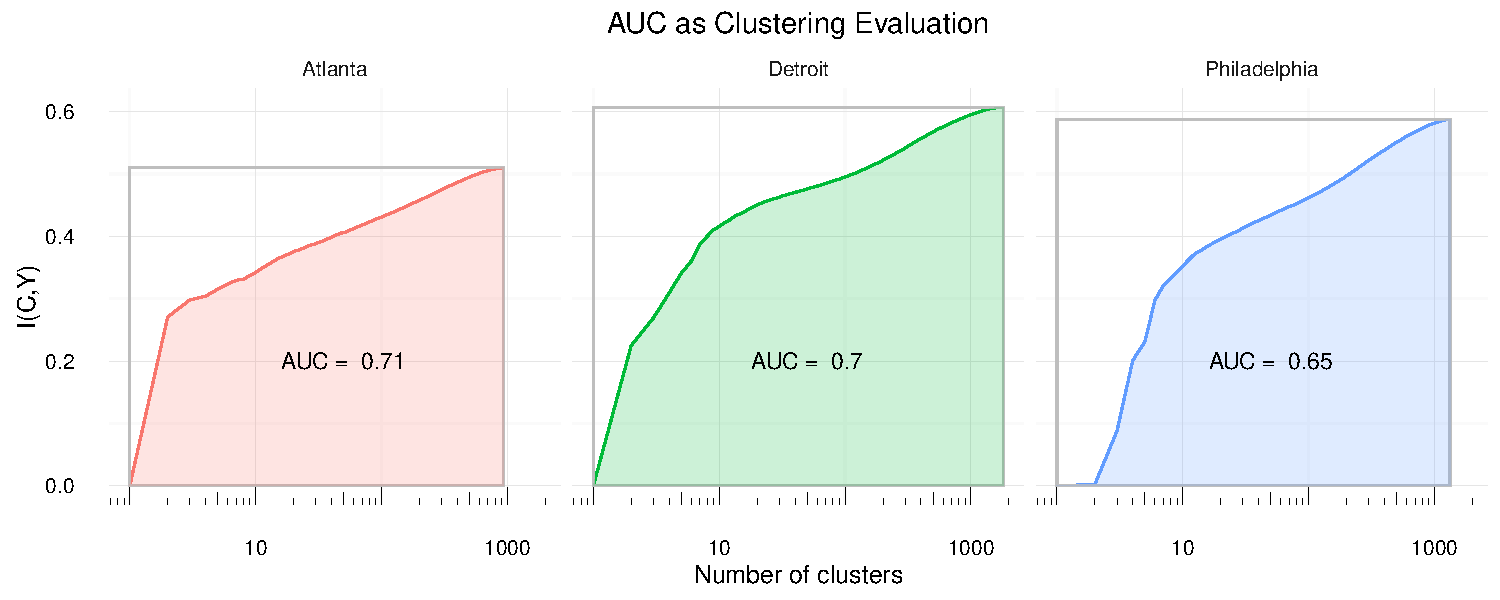
\includegraphics[width=\linewidth]{figs/AUC_illustration.pdf}
			\caption{
				Evaluation of clusterings using the area under the curve (AUC) for $\mathcal{Y} = \{\text{Black }, \text{Non-Black}\}$, computed according to the formula \eqref{eq:AUC_formula}. 
				The bounding rectangle for each city is shown in grey. 
				The AUC is the proportion of the rectangle contained in the shaded region. 
				The AUC for Philadelphia has been adjusted to account for the data set's two disconnected geographic components.
			} \label{fig:AUC}
	\end{figure}
	\begin{figure}
		\centering
		\input{figs/adjusted_regression.txt}
		\caption{
			Regression of the AUC computed by \eqref{eq:AUC_formula} on the information measures $H(Y)$, $I(X,Y)$, and $J(X,Y)$. 
			95\% confidence intervals for each of the determined coefficients are shown in parentheses. 
			The three information measures jointly explain an adjusted 75\% of the variation in the AUC. 
		}\label{fig:regression}
	\end{figure}

\section*{Discussion}


\matmethods{Please describe your materials and methods here. This can be more than one paragraph, and may contain subsections and equations as required. Authors should include a statement in the methods section describing how readers will be able to access the data in the paper. 

\subsection*{Subsection for Method}
Example text for subsection.
}

\showmatmethods{} % Display the Materials and Methods section

\acknow{P.C. is grateful to Marta C. Gonz\'{a}lez for helpful discussion, and to MIT-Saudi Arabia...}

\showacknow{} % Display the acknowledgments section

% \pnasbreak splits and balances the columns before the references.
% Uncomment \pnasbreak to view the references in the PNAS-style
% If you see unexpected formatting errors, try commenting out \pnasbreak
% as it can run into problems with floats and footnotes on the final page.
% \pnasbreak

\nocite{Bettencourt2013}

% Bibliography
\bibliography{/Users/phil/bibs/library.bib}

\end{document}